% Chapter 2

\chapter{Background} % Main chapter title

\label{Background} % For referencing the chapter elsewhere, use \ref{Chapter1} 

\lhead{Chapter 2. \emph{Background}} % This is for the header on each page - perhaps a shortened title

This chapter serves an introductory purpose, since an extensive analysis to all the specific research components of this thesis is following. First, evolutionary algorithms and robotics are discussed in depth. More specifically, genetic algorithms are presented, the role of the encoding in an evolutionary setting,  how artificial neural networks can represent an organism in an EA, and how these ANNs can be evolved coupled with an evolutionary algorithm. As part of the different encoding schemes, an indirect coding called compositional pattern producing networks is also discussed in detail. The aspect of the objective function in such problems and the affect that has in the performance, additionally a search that uses an objective function that rewards diversity in the evolution is presented. Last, a field of robotics and material sciences, soft robotics is investigated in conjunction with ways that these soft material structures can be simulated in a virtual environment.


\section{Evolutionary Robotics}

Evolutionary robotics~\cite{WikievolutionaryRobotics} (ER) is a method that makes use of evolutionary computation algorithms to develop (evolve) robots controllers, without the direct programming by humans. One big advantage of this method is that it can evolve controllers for robots for environments that human designers and engineers do not have enough knowledge about (i.e., designing a robot controller for another planet, where surface type and gravity level might be crucial variables for the design of an exploring robot). In the same fashion as natural evolution, evolutionary techniques work with a population of random initialized controllers. The candidate population individuals (robot controllers) used in ER applications may be drawn from some subset of the set of artificial neural networks (ANNs), whereas simpler versions of genetic algorithm applications use \texttt{bit}-\texttt{float}-\texttt{integer} streams that directly represent a controller. The controllers in the better performing robots are selected then, altered and propagated through mutation, crossover, and other genetic operations, in a repeating process that mimics natural evolution. Evolutionary robotics is done with many different objectives, often at the same time. These include creating useful controllers for real-world robot tasks, reproducing biological phenomena, etc.. Creating controllers via artificial evolution requires a large number of evaluations of a large population. This is usually takes a lot of computational time, which is one of the reasons why evolution of such controllers is usually evaluated within a simulation software. Also, initial random controllers may exhibit potentially harmful behaviour, such as repeatedly crashing the robot into a wall, which may damage a physical robot.

Apart from evolutionary methods to develop robot controllers reinforcement learning is used, rewarding actions, which translates to state-action pairs that lead to high rewarding behaviors, as a result, a robot controller can be indirectly built.

Applying evolved robot controllers to real robots in a physical environment is an extremely difficult task, since simulators in front of the limitations of computing efficiency sacrifice the accuracy.

In some cases, evolutionary methods can be used to design the physical structure (morphology) of the robot~\cite{hiller2010evolving}, in addition or in place of the controller. This thesis is exploring that aspect of evolution.

Developmental robotics is a field related to evolutionary robotics,  while instead of evolving through generations towards more fit controllers, it is trying to mimic life-like learning starting from a ``blank'' state in which the robot's ``brain'' is initialized and everything is unknown.


\section{Evolutionary Algorithms}

Evolutionary algorithms were discussed as part of the process of evolutionary robotics in the previous section, and it only refers to the algorithms that evolves the controllers. In this section several aspects of evolutionary algorithms, mostly in respect of how the ``brain'' is represented in the solution space (i.e, encoding), will be discussed extensively.


\subsection{Genetic Algorithms}
Genetic are in principle part of the evolutionary algorithms and follow the same principles.

\begin{quote}Genetic algorithms are probabilistic search procedures designed to work on
large spaces involving states that can be represented by strings.\end{quote}

Considering the above quote by~\cite{goldberg1988genetic}, a genetic algorithm is a process of evolving a stream of values, which is a single solution in a high dimensional problem space. These values can be at their simplest form, bit ($0, 1$), integer, or float values. 

Each of these solutions is called a \emph{phenotype}, and the stream the solution is derived from, \emph{genotype} or \emph{chromosome}. Genetic algorithms are also a type of evolution based on generations. Each generation holds a population of individuals which are initially randomly selected out of a distribution in the solution space. The iterative process that follows and creates, given the current population of individual genotypes, the new population, is called \emph{generation}. Usually the algorithm terminates after a fixed step of generations or when the goal has been reached. 

The way the next generation's population is produced completely depends on the current population, genotypes are selected to breed new individuals. There two basic ways of how a new genotype is going to be produced. The first way is called \emph{mutation} and requires only one individual from the current population. Mutation will change one or more values in the \emph{chromosome} of the selected individual to create a new one and maintain the genetic diversity from one generation to the other. \emph{Crossover} is the second basic genetic operator and requires two or more parents for each new individual. This operator is similar to biological crossover and it uses parts from all parents to create a new chromosome.

The way individuals are selected after each successful generation in order to produce new individuals, belongs to the process of \emph{selection}. Selection, as the name reveals itself, selects which individuals will become parents and which individuals will not. The selection criteria, as it also happen in some natural environments where the most fit organisms survive, is a function that can approximate how good is an individual. This \emph{objective} function, also called \emph{fitness}, is a measure of how good an individual is (i.e. total displacement of a robot's body while trying to evolve walking). With the knowledge of the fitness function added to the evolution, weak individuals can be discarded from the breeding process. Selecting parents randomly from the top part of the population or selecting parent via \emph{tournament}, known also as \emph{competition} (i.e., multiple random picks of individuals from the whole generation's population keeping the best pick) are two of the basic selection methods in evolutionary algorithms.


\subsubsection*{Direct-Indirect Encoding of the Genotype}

\begin{figure}
\centering
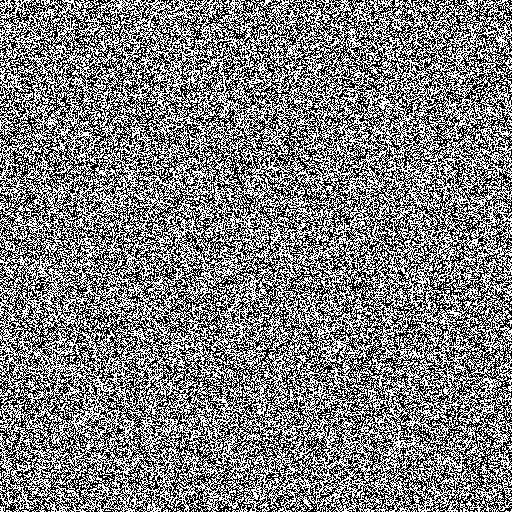
\includegraphics[width=0.3\textwidth]{../Figures/Misc/direct.jpg}\  \   \   
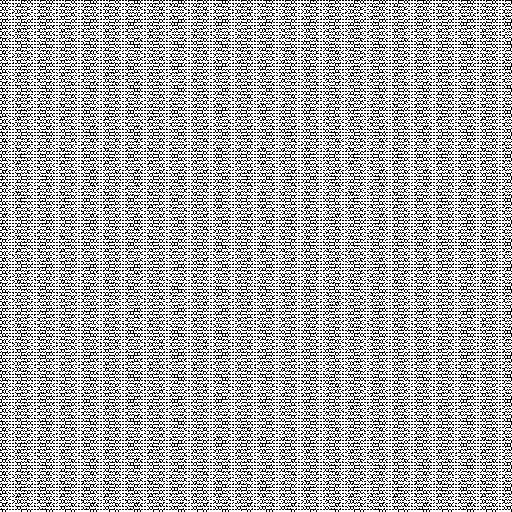
\includegraphics[width=0.3\textwidth]{../Figures/Misc/indirect.jpg}
\caption{Comparison \emph{direct} encoding versus \emph{generative} for the binary image example.}
\label{fig:directVsIndirectEncoding}
\end{figure}



A simple direct coding was described in the previous part that a single dimension stream of bits or numbers describe the chromosome. When the dimensions of the task define the length of this genome, we have a \emph{direct} encoding, which means that the genotype-phenotype mapping is direct. An example of that case could be the design of a two dimensional binary image. In direct encoding the genotype of this picture can be represented by a stream of bits which has the same length as the image's pixels. In other cases and when there is no direct mapping between the genotype and the phenotype, indirect encoding is presented. For the same example, in indirect encoding the genotype would be represented by a function that give pixel values $0$ or $1$ for every pixel's coordinate. Figure~\ref{fig:directVsIndirectEncoding}, illustrates the difference between direct and indirect encoding, an example binary image is shown for both encoding schemes, in the first case (direct) the genotype is a binary stream which length is the equal with the number of pixels producing the value of each pixel directly. The latter encoding, uses a genome of length 3, as many as the coefficients of a linear combination of the function that involves $sin, cos, tan$-functions, the result is taken after applying the same function for each pixel coordinate. Even when a simple function is used the  phenotype holds some of its functions properties such as symmetry and repetition, resulting in a pattern than no direct encoding can match. On the other hand, direct encoding cannot produce anything noticeable.



\subsection{Compositional Pattern Producing Networks}


\begin{figure}
\centering
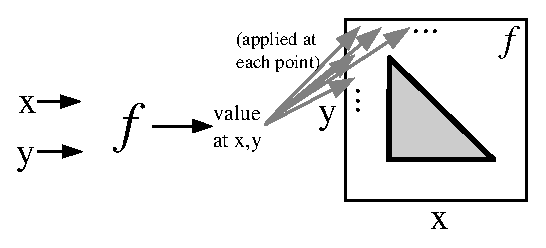
\includegraphics{../Figures/Misc/cppnResolution.eps}
\caption{CPPNs work as a function $f$ that is being queried for the whole n-dimensional Cartesian space in which space maps the phenotype, in this case the phenotype is the triangle, figure taken by~\cite{stanley2007compositional}.}
\label{fig:cppnResolution}
\end{figure}



Encoding plays an important role and it is critical about the performance of evolutionary algorithms ecpecially when huge problem spaces are present. Research have shown that the genotype-phenotype mapping can affect performance~\cite{komosinski2001comparison}. More than that, the geometrical implications of the problem also have some potentially important role in the encoding problem. Thus, the role of symmetry to machine learning technique is important~\cite{gauci:aaai08}, especially in applications like board games, robot controllers, biped walking, etc., where geometric regularities can be descriptive about the nature of the problem.



\begin{figure}
\centering
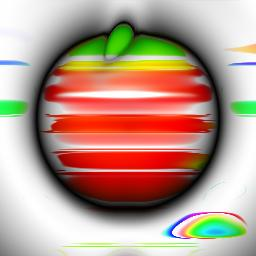
\includegraphics[width=0.25\textwidth]{../Figures/Misc/picBreed3.jpg}\  \   \   
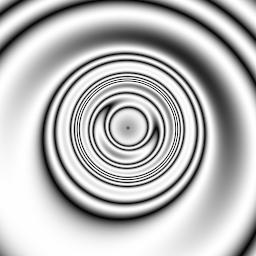
\includegraphics[width=0.25\textwidth]{../Figures/Misc/picBreed1.jpg}\  \   \   
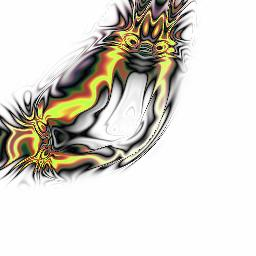
\includegraphics[width=0.25\textwidth]{../Figures/Misc/picBreed2.jpg}
\caption{Compositional pattern producing networks can encode truly complex structures and shapes in the phenotypic level. Source~\cite{picbreederSite}.}
\label{fig:cppnImages}
\end{figure}



\emph{Compositional pattern producing networks}~\cite{stanley2007compositional} or CPPNs are artificial neural networks in their base with an extended set of activation functions. Results by this encoding show that repetitive and structural patterns can be produced in this generative mapping from the genotype to the phenotype space. Just like in the previous two dimensional image representation of a phenotype, CPPNs generate phenotypes that can be interpreted as distributions of points in a multidimensional Cartesian space. The genotype (CPPN) can be then queried for each coordinate of the space and give the phenotype representation of the genotype in multiple resolutions. In the same fashion, images can be constructed using CPPNs, where pixel coordinates are queried to the network and the grayscale-RGB values can be taken by the outputs of these networks. Figure~\ref{fig:cppnImages}, illustrates images encoded by CPPNs. Comparing the results with figure~\ref{fig:directVsIndirectEncoding}, is now understandable why this kind of encoding can perform better in cases that symmetry is important.

Figure~\ref{fig:cppnResolution}, illustrates how the mapping between the genotype and phenotype is done using generative encoding like CPPNs. A major asset of CPPNs is that they can generalize in all kind of resolutions. Considering the previous figure again, the CPPN is queried for all $x,y$ coordinates of the phenotype two dimensional Cartesian space. The step of $x,y$ sampling can be determined by the problem, since the inputs of the CPPN are the normalized coordinates $x,y \in [-1,1]$. Thus, genotypes using this kind of generative encoding can be mapped in every resolution, making it straightforward to generalize into larger spaces.

Compositional pattern producing networks have used in many applications where symmetry and repetition can produce artistic three or two dimensional structures\cite{endlessforms}, or drawings~\cite{secretan2008picbreeder,picbreederSite}.



\subsection{Neuroevolution}
\emph{Neuroevolution} is an optimization technique using evolutionary methods as described above, whereas artificial neural networks take the place of simpler representations from the genotype (bit-streams) to the solution space. ANNs can compute arbitrarily complex functions, learn and perform under the presence of noisy inputs and generalize to unseen sensory information. Neuroevolution requires only a measure of a network's performance at a task. This more complicated form of chromosome representations can develop more complex ``brains'' for robot controllers. After each run, the sensory input of the task domain is given at the artificial neural network's input neurons, and the solution is given by the network's outputs, where the fitness of the specific ``brain'' can be evaluated. A major issue is the selection of the network's \emph{topology}, topology is the arrangement of the network's elements such as links and nodes, which represents the structure and how the information flows within the network. In early neuroevolution implementations the topology of the networks used, was fixed, meaning that the only elements of the networks evolving were the weights of the connections between the nodes.





\subsection*{Neuroevolution of Augmented Topologies}

Neuroevolution of augmented topologies (NEAT) as it first introduced by~\cite{stanley2002evolving} is a method of evolving neural networks, which evolves the topologies of the networks alongside its weights.

Originally, neuroevolution methods (methods that evolve ANNs), developed to capture difficult sequential decision as well as control problems, where sensory information is the input of these neural networks and decision are the outputs. NEAT is another method for evolving ANNs, whereas a few simple features are added, making it able to find solutions in more demanding problems. NEAT starts the evolution process with a population of networks with simple topologies. Through the generations instead of just fixing the weights of the networks' connections, topologies will become more complex allowing nodes and links to be added along the generations. Meaning that during evolution, more complex networks will be produced, this \emph{complexifying} technique leads to capture more demanding problems, as it offers enough freedom to the evolution.

Several aspects of this method worth mentioning, with \emph{speciation} be the most important one. Speciation is the procedure that protects new \emph{species} until the have enough time to evolve, before comparing them with the rest of the population. For two individual genotypes (ANNs) to belong to the same species, their network topology must be similar, meaning that a threshold is set, and a function determines the numeric value of two network topologies' similarity. The age of each species protects them for competing in equal terms with more optimized species, giving them in this way time to evolve further towards the objective function.



\subsection*{CPPN-NEAT}

Neuroevolution of augmented topologies is an evolutionary algorithm which not only evolves artificial neural networks but also their topology along. Compositional pattern producing networks are identical to ANNs in respect to their structure, also can make use of the \emph{complexifying} property, capturing in this way regularities in more complex problems. NEAT method can likewise evolve CPPNs in the place of ANNs, since it only needs minor modifications.

The resulted method that evolves this generative type of genomes (CPPNs) is called CPPN-NEAT~\cite{stanley2007compositional}, and its only difference is in the way new nodes are added to the networks. Originally NEAT used to evolve ANNs which are using sigmoid functions to every node, so it was a trivial solution that every new-added node will carry this function, on the other hand CPPNs use functions from a canonical set, whereas CPPN-NEAT assigns a random function from this set to every newly added node.

Experiments have shown that the discussing method can indeed evolve CPPNs, capturing like this solutions in problems with geometrical nature, holding alongside essential properties of natural evolution. Furthermore, neuroevolution of CPPNs can also determine the connectivity patterns of neural networks in NEAT method~\cite{stanley2009hypercube}.




\section{Novelty Search}

Traditional search within the framework of evolutionary algorithms need an objective function, a function that leads the search towards ``good'' areas of the solution space, following the gradient of the fitness. Defining the fitness function is a straightforward problem most of the times, in a problem when a robot tries to get from its initial position to a target position in a room with no obstacles in between, a fitness function could be determined as the euclidean distance between the final position of the robot and the target point, the closer it gets to the target the more points (higher fitness) the specific controller is rewarded.

\subsubsection*{When the objective function lies}

\begin{figure}
\centering
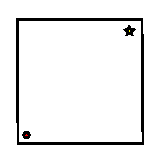
\includegraphics[width=0.3\textwidth]{../Figures/Misc/mazeEasy.eps}\  \ \   \   
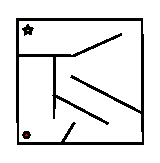
\includegraphics[width=0.3\textwidth]{../Figures/Misc/maze.eps}
\caption{Objective functions can be devious. Maze example from~\cite{lehman2011abandoning}.}
\label{fig:maze}
\end{figure}

Such a measure as the objective function, is not always truthful, in fact, following the gradient of fitness in many problems can lead to local optima, misleading the search, which eventually stacks in these localities of the problem without performing any more exploration. 

Considering the robot-maze example presented in~\cite{lehman2011abandoning,lehman2010revising}, a robot (red dot) is placed in a maze (fig.~\ref{fig:maze}), the robot has sensory information which are inputs to its controller (``brain''), the controller is driving the robot through the maze having only radar sensor information, when its ultimate goal is to drive the robot to the target position (star) in a fixed time span. Naturally, to select a fitness function that can give enough information about how good a controller is, the euclidean distance to the target from the final position of the robot in the end of the simulation time is measured, providing knowledge to the search. For the first maze (left) when no obstacles are between the robot and its target, the objective function is reliable, since the euclidean distance to the target indeed informs the robot how close it is located. In the second maze (right), using the previous objective function, things are not straightforward. In this example maze, achieving high fitness does not mean that the robot is actually close to the target. Driving north in this maze following the fitness gradient leads to a wall that cannot be passed by the robot, thus, exploration is needed in low-fitness areas which will allow the robot to reach the target point with the maximum fitness. The deceptive nature of the fitness function in this problem can be found in a lot of optimization problems, and the walls in this maze clearly denote problems where this fitness landscape can be found.

\subsubsection*{Natural evolution is not a search for fitness}

Using an objective function in evolutionary computation and typically reward individuals which are closer to an objective, is far away from natural selection in the evolution process, where exploration is allowed as long as, the criteria for survival hold~\cite{lehman2010revising}. Driving search towards promising parts of the fitness space, whereas local optima may be present, ensures that other areas of the search will not be explored, leading the search to stay and explore the nearby area, while more promising regions are far away in solution space. Solutions located in these regions are called \emph{stepping stones}~\cite{lehman2008exploiting,lehman2011abandoning,lehman2010revising,risi2009novelty} and are points in the search space that may not be good, as far as their objective values is concerned, but can eventually lead to better or a global optima.


\subsubsection*{Search for Novelty}

\emph{Novelty} search~\cite{lehman2008exploiting,lehman2011abandoning,lehman2010revising, risi2009novelty} unlike traditional fitness-based search is an alternative way of optimization towards an objective function without having knowledge of this objective. In simple words, it is looking for a solution to a problem without knowing how close it is to actually solve it, which turns out to be a major impact to the increased performance of this method in several domain problems. A similar concept can also be found in reinforcement learning when the need for exploration has to be preserved through the learning process.

What novelty search seeks for, is how interesting is a new solution in respect to all previously found ones. To define ``interesting'' we need to move our point of interest into behavioral space, which is a function of each phenotype just like the fitness. Nevertheless, it fully describes the behavior without implying directly the fitness function. As an example someone can think of, the final position of the navigation robot, or the trajectory of it, in the previous robot-maze example. Rewarding behaviors of the phenotype that are different from the previously found, evolution is being driven to visit new points in the behavior search space.

One significant point here is that the behavioral space in some domains can be limitless. However, a valid behavioral metric could be found, excluding behaviors that are meaningless or do not comply with the natural limits of the problem. Additionally, enumerating all possible solutions in the behavior space is similar to a brute force approach which could have the same results. On the other hand, the genotype's search space can be also infinite, especially in neuroevolution methods like NEAT, in where ANNs can grow over evolution time. A bounded space of understandable behaviors is then the key idea of novelty search, whereas increasingly complex behaviors present to the evolution as the complexity of the genotype grows along.

Multi-objective optimization can also make use of novelty metric trying to optimize both objectives fitness and novelty at the same time~\cite{mouret2011novelty}. Another method that exploits the diversity of the produced genomes in order to map the phenotype to the fitness is also proposed by the literature~\cite{mouret2012algorithm}.

\subsubsection*{Is novelty search the similar to random?}

Initial thoughts are converging that novelty search is completely random search, constantly looking for something new in the vast space of behaviors is similar to evolving random robot controllers without caring about behavioral aspect of their phenotypes, hoping that enough exploration will be done in both genotype and phenotype spaces. Thus, having no information about the actual behaviors the evolved phenotypes produce, can harm the evolution as different and more complex genotypes can easily produce similar behaviors. The novelty in behavior level assures that the search will explore deeply the behavioral space with the hope that a \emph{fit} behavior will be found. Aside from that, novelty search does not perform backtracking which ensures that it will constantly drifts away from already found behaviors, in the same time, there is no such guarantee in random search. Therefore, it is certain, that no exploration in the behavior space will be performed by random search.



\subsubsection*{How novelty can be measured}

As fitness is a function to measure the ``goodness'' of an individual, novelty measures how different is an individual against all previous found by the evolution. To define different, novelty metric measures the difference in the behavioral space of the phenotype. Given the phenotype's behavior $x$, a novelty measurement could be a function of $x$, $f(x)$, which computes how different (novel) is the specific behavior in respect to a set of other behaviors $S$ in behavior space.  As defined in~\cite{lehman2008exploiting,lehman2011abandoning}, \emph{sparseness} can give a good measurement of how sparse is the area of a newly introduced behavior. Given the behavior, we can compute the sparseness by:
\begin{equation}
\label{sparsenessEquation}
f(x) = \cfrac{1}{k} \sum_{i=1}^{k} d(x, S_i)
\end{equation}
, where $S$ is a sorted set of the closest behaviors, so that the average distance from the $k$-closest behaviors.


\subsubsection*{Algorithm}

There is no need of extensive modification in any evolutionary algorithm in order novelty search to be implemented, apart from replacing fitness with a novelty measure. To push search to visit new areas in the behavior space we need to reward every novel behavior coming up during the evolution. For this reason, storing novel reference points in space (behaviors) during the evolution seems logical. The sparseness of a new behavior is computed by equation~\ref{sparsenessEquation}, resulting in a numerical value that implies how novel is the found behavior. If the new behavior has a novelty value more than this threshold it is also stored in the novel individuals' population. Apart from comparing any new behavior with all the novel stored ones, the newly produced can also be confronted with the entire set of behaviors produced in the same generation of the evolution.



\section{Soft Robotics}
As the name suggests soft robots~\cite{trivedi2008soft, pfeifer2012challenges} are made completely of soft materials mimicking animals or animal-parts that consist of soft tissue (elephant trunk, tongue, worm, octapus, etc.). Having no rigid parts, the degrees of freedom can explode and the possible ways of motion can become extremely complicated. In traditional robotics, joints and rigid parts predefine the set of possible movement space and sometimes restrict the robot's locomotion strategy to a specific gait set. In soft robotics, the absence of rigid parts can on the one hand make the design of the locomotion strategy exceptionally tortuous, on the other hand though, the gait alternatives are limitless.

\begin{figure}[t!]
\centering
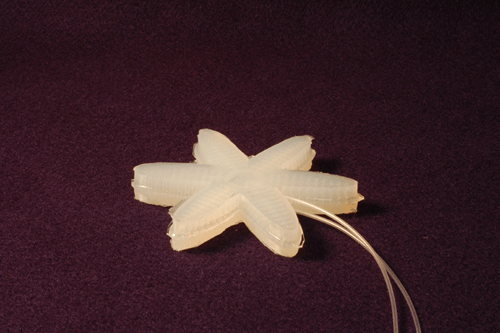
\includegraphics[width=0.3\textwidth,height=0.13\textheight]{../Figures/Misc/soft_robotics_figure.png}\		
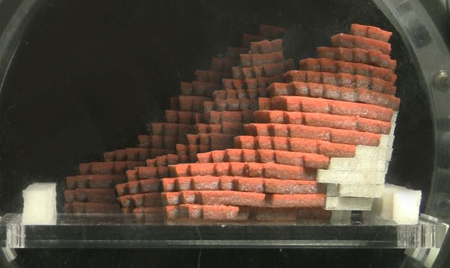
\includegraphics[width=0.3\textwidth,height=0.13\textheight]{../Figures/Misc/hillerPressureChamber.png}\	
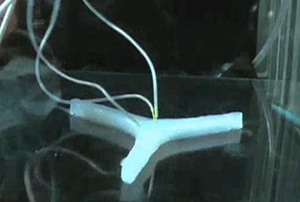
\includegraphics[width=0.3\textwidth,height=0.13\textheight]{../Figures/Misc/ExplodingRobot.jpg}\\
\caption{Soft robots can be actuated through air pressure tubes (left), pressure variation (middle), even internal explosions (right).}
\label{fig:softRobotsActuation}
\end{figure}

Actuating soft materials can be done in many ways including pneumatic systems~\cite{ilievski2011soft, shepherd2011multigait}, hydraylic, internal body explosions, pressure tubes, temperature changes and others~\cite{laschi2012soft, seok2010peristaltic}. Figure~\ref{fig:softRobotsActuation} illustrates some actuating soft robots. 

It may seem immature, nevertheless, soft robotics research field is growing fast. Some of their characteristics make them interesting to explore, such as the infinite number of degrees of freedom, the variety of materials (mostly elastic) that can be used in the contrary to rigid robotics that are mostly made out of metals and plastic. Nevertheless, structure design and control of soft robotics remain challenging mostly because of their soft bodies can only be represented in continuous state space, where only analytical methods can prove successful.

To sum up, a lot of research is being done in the field of soft robotics and materials, locomotion capabilities of soft robots as well as the fact that can passively move makes them an interesting topic for present and future research. Finally, considering also that soft materials can be more friendly than conventional robot materials to humans, human-robot interaction can become in this way safer~\cite{sanan2011continuum}.


\subsection{Soft Robotics in Simulation}

Most work to simulate interactions and deformations within and between soft material bodies are mostly focused on the graphical part of the problem, sacrificing the accuracy of the simulation. Three dimensional meshes can represent these bodies including their dynamics of their materials. 

A recent work though, \emph{VoxCad} simulator~\cite{hiller2012dynamic}, is focusing mostly on the engineering side of the soft material interactions, not at the expense of a low frame rate. \emph{VoxCad} is a modeling and analyzing open-source software that can simulate soft material deformations and interactions. In figure~\ref{fig:VoxCAD}, VoxCad software is illustrated during the simulation of the soft robot depicted in the simulator.

VoxCad cannot model and simulate three dimensional meshes, yet a lattice is used to represent the 3D workspace where voxels (three dimensional pixels) can be assigned different materials. Materials have properties such as the elasticity of the material, density, Poisson's ratio, coefficient of thermal expansion (which determines how materials will be expanded in respect to the environment's temperature), temporal phase in respect to the temperature period, and the friction coefficients to the ground. Materials can also be mixed together to create a new type of material.

Materials themselves are passive and cannot actuate without external trigger. In this simulator this external force that can actuate the materials is the temperature of the environment. The main variables of the environment is the base, the amplitude and finally, the period of the temperature. Furthermore, the gravity acceleration of the environment can vary.

Throughout this thesis, a structure or a soft robot will refer to a set of connected voxels (not unconnected parts) within the lattice space. For universal or experimental settings used during the simulations you can see Appendix~\ref{AppendixA}.



\begin{figure}
\centering
\includegraphics[width=1.0\textwidth]{../Figures/Misc/voxcad.png}
\caption{VoxCAD (Voxel CAD),a cross-platform open source voxel modeling and analyzing software.}
\label{fig:VoxCAD}
\end{figure}

\section*{\todo{Additional Material that can be added later}}

\cite{stanley2003taxonomy}
\cite{nelson2009fitness}
\cite{meyer1998evolutionary}
How the Body Shapes the Way We Think A New View of Intelligence~\cite{pfeifer2007body}
\cite{albu2008soft}
\cite{woolley2011deleterious}
\cite{lewis1992genetic}
\cite{lapeyre2011maturational}
\cite{oudeyer2013intrinsically}
\cite{gauci:gecco07}
